
% Standalone TikZ/PGFPlots figure for "Channel weighting for temporal smoothness"
% Professional design with wider bars, better spacing, improved readability
% Compile with: xelatex -interaction=nonstopmode temporal-weights.tex

\documentclass[tikz,border=15pt]{standalone}
\usepackage{pgfplots}
\pgfplotsset{compat=1.18}
\usepackage{fontspec}
\usepackage{microtype}

\begin{document}
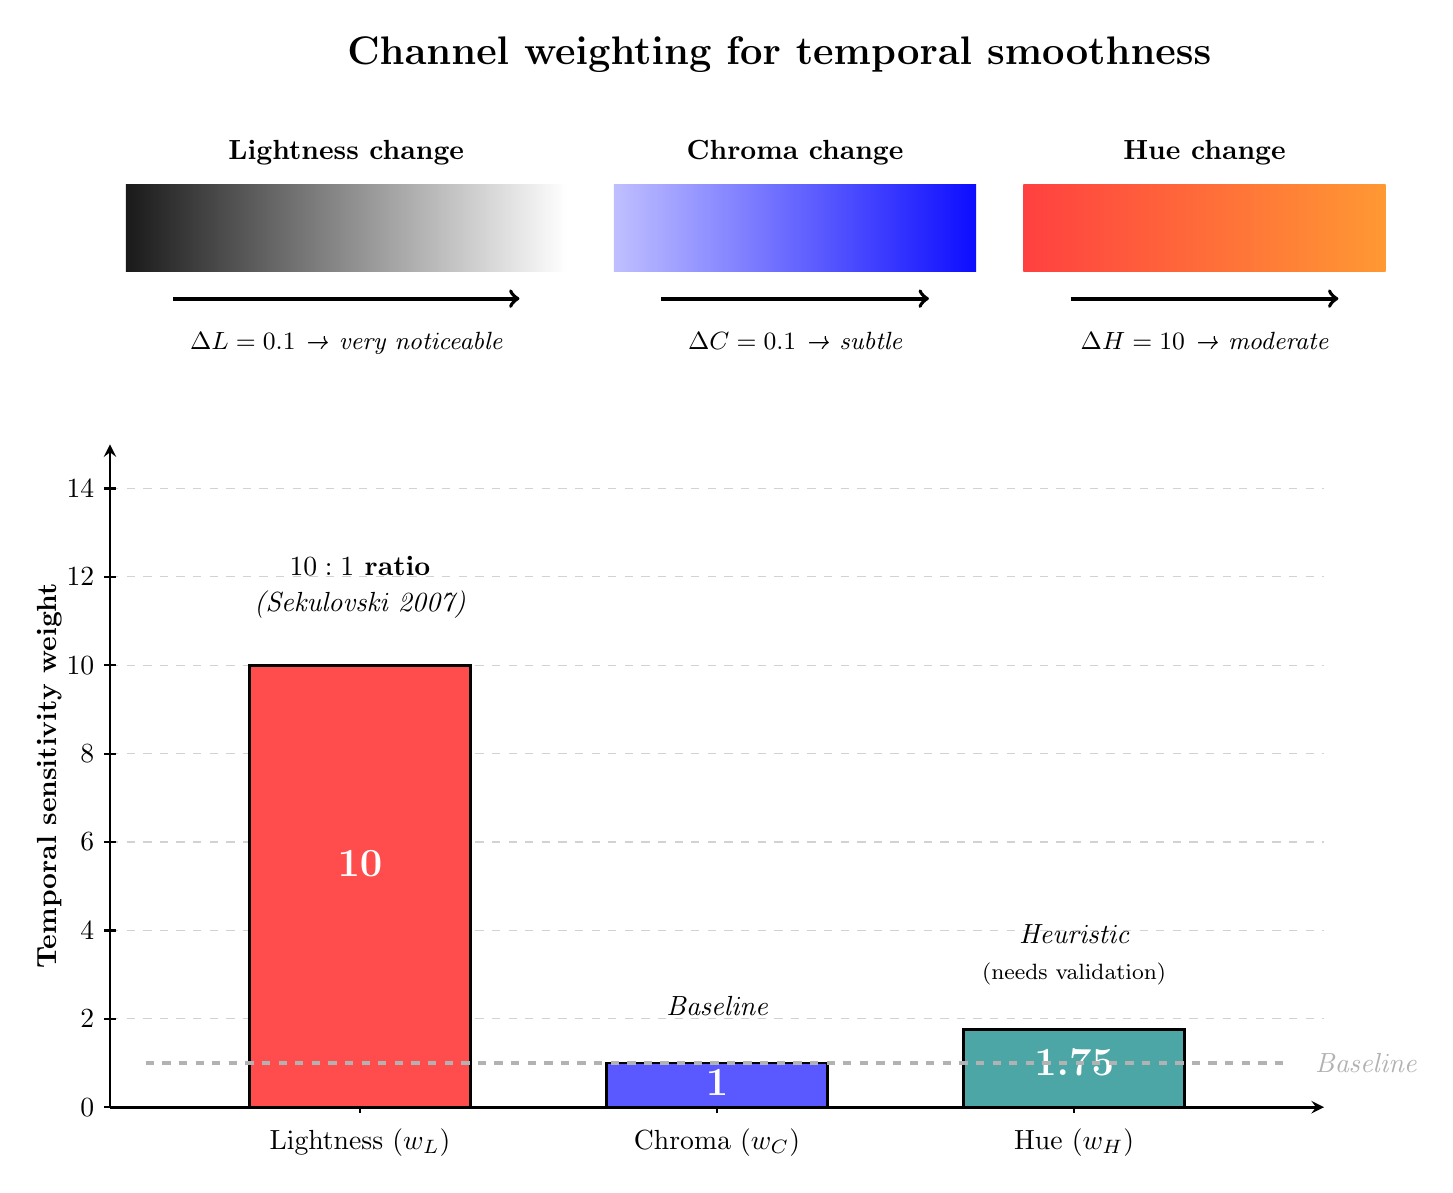
\begin{tikzpicture}

  % ===== TOP SECTION: Gradient swatches showing perceptual changes =====
  \begin{scope}[yshift=1.8cm]
    % Main title with more space below
    \node[font=\Large\bfseries, anchor=south] at (8.5, 2.8) {Channel weighting for temporal smoothness};
    
    % ───── Lightness swatch ─────
    \shade[left color=black!90, right color=white] (0.2, 0.4) rectangle (5.8, 1.5);
    \node[anchor=south, font=\normalsize\bfseries] at (3.0, 1.62) {Lightness change};
    \draw[->, line width=1.4pt, color=black] (0.8, 0.05) -- (5.2, 0.05);
    \node[anchor=north, font=\small\itshape] at (3.0, -0.25) {$\Delta L = 0.1$ → very noticeable};
    
    % ─── Chroma swatch (blue gradient) ───
    \shade[left color=blue!25, right color=blue!95] (6.4, 0.4) rectangle (11.0, 1.5);
    \node[anchor=south, font=\normalsize\bfseries] at (8.7, 1.62) {Chroma change};
    \draw[->, line width=1.4pt, color=black] (7.0, 0.05) -- (10.4, 0.05);
    \node[anchor=north, font=\small\itshape] at (8.7, -0.25) {$\Delta C = 0.1$ → subtle};
    
    % ───── Hue swatch (red→orange gradient) ─────
    \shade[left color=red!75, right color=orange!80] (11.6, 0.4) rectangle (16.2, 1.5);
    \node[anchor=south, font=\normalsize\bfseries] at (13.9, 1.62) {Hue change};
    \draw[->, line width=1.4pt, color=black] (12.2, 0.05) -- (15.6, 0.05);
    \node[anchor=north, font=\small\itshape] at (13.9, -0.25) {$\Delta H = 10°$ → moderate};
  \end{scope}
  
  % ===== BOTTOM SECTION: Bar chart with wider bars and better spacing =====
  \begin{axis}[
    at={(0, 0)},
    anchor=north west,
    width=17cm,
    height=10cm,
    xmin=0.3,
    xmax=3.7,
    ymin=0,
    ymax=15,
    ymajorgrids=true,
    grid style={dashed, gray!35},
    xtick={1, 2, 3},
    xticklabels={Lightness $(w_L)$, Chroma $(w_C)$, Hue $(w_H)$},
    xticklabel style={font=\normalsize, yshift=-2pt},
    ylabel={Temporal sensitivity weight},
    ylabel style={font=\normalsize\bfseries, yshift=-5pt},
    axis x line=bottom,
    axis y line=left,
    axis line style={line width=1pt},
    tick style={draw=black, line width=0.8pt},
    x tick label style={align=center},
    ytick={0, 2, 4, 6, 8, 10, 12, 14},
    scaled y ticks=false,
    bar shift=0pt,
    clip=false
  ]
    % Bar 1: Lightness - centered on tick
    \addplot[
      ybar,
      draw=black,
      line width=1pt,
      fill=red!70,
      mark=none,
      bar width=80pt
    ] coordinates {(1, 10.0)};
    
    % Bar 2: Chroma - centered on tick
    \addplot[
      ybar,
      draw=black,
      line width=1pt,
      fill=blue!65,
      mark=none,
      bar width=80pt
    ] coordinates {(2, 1.0)};
    
    % Bar 3: Hue - centered on tick
    \addplot[
      ybar,
      draw=black,
      line width=1pt,
      fill=teal!70,
      mark=none,
      bar width=80pt
    ] coordinates {(3, 1.75)};
    
    % Value labels inside bars - larger and better positioned
    \node[font=\Large\bfseries, white] at (axis cs:1, 5.5) {10};
    \node[font=\Large\bfseries, white] at (axis cs:2, 0.55) {1};
    \node[font=\Large\bfseries, white] at (axis cs:3, 1.0) {1.75};
    
    % Source/evidence annotations above bars
    \node[
      font=\normalsize,
      anchor=south,
      align=center,
      inner sep=4pt
    ] at (axis cs:1, 10.8) {\bfseries $10:1$ ratio\\[1pt]\normalfont\itshape(Sekulovski 2007)};
    
    \node[
      font=\normalsize\itshape,
      anchor=south,
      align=center,
      inner sep=4pt
    ] at (axis cs:2, 1.8) {Baseline};
    
    \node[
      font=\normalsize,
      anchor=south,
      align=center,
      inner sep=4pt
    ] at (axis cs:3, 2.5) {\itshape Heuristic\\[1pt]\normalfont\footnotesize(needs validation)};
    
    % Reference baseline at y=1.0
    \draw[gray!60, dashed, line width=1.2pt] (axis cs:0.4, 1.0) -- (axis cs:3.6, 1.0);
    \node[
      font=\normalsize\itshape,
      gray!60,
      anchor=west,
      inner sep=3pt
    ] at (axis cs:3.65, 1.0) {Baseline};
    
  \end{axis}

\end{tikzpicture}
\end{document}

